% ================================================================
% The cocoa price shock and Swiss chocolate - consulting-style deck (16:9)
% Compile: xelatex Deck_Cocoa_Shock_Swiss_Chocolate.tex (twice)
% Font: TeX Gyre Heros (GUST Font License), shipped in ../fonts/
% ================================================================
\documentclass{article}
\usepackage[paperwidth=338.67mm,paperheight=190.5mm,margin=0mm]{geometry}
\usepackage{fontspec}
\IfFileExists{../fonts/texgyreheros-regular.otf}{%
  \setmainfont{texgyreheros-regular.otf}[Path=../fonts/, BoldFont=texgyreheros-bold.otf,
    ItalicFont=texgyreheros-italic.otf, BoldItalicFont=texgyreheros-bolditalic.otf]
}{\IfFontExistsTF{Helvetica}{\setmainfont{Helvetica}}{\setmainfont{TeX Gyre Heros}}}
\usepackage{xcolor,graphicx,tikz,enumitem,tabularx,booktabs,microtype}
\usepackage[document]{ragged2e}
\pagestyle{empty}
\definecolor{blue}{HTML}{2A78D6}
\definecolor{orange}{HTML}{EB6834}
\definecolor{ink}{HTML}{1F1F1E}
\definecolor{ink2}{HTML}{52514E}
\definecolor{rule}{HTML}{E4E2DC}
\definecolor{tint}{HTML}{EEF4FC}
\definecolor{tintor}{HTML}{FDF0EA}
\color{ink}
\setlength{\parindent}{0pt}\setlength{\parskip}{0pt}
\setlist{nosep,leftmargin=1.1em,itemsep=7pt,label={\color{blue}\textbullet}}
\newcommand{\mn}{\char"2212\relax}
\hyphenpenalty=5000

% slide frame: #1 action title, #2 source line, #3 body; page number from counter
\newcounter{slide}
\newcommand{\slide}[3]{%
  \stepcounter{slide}%
  \begin{tikzpicture}[remember picture,overlay]
    \node[anchor=north west,inner sep=0pt] at ([xshift=18mm,yshift=-13mm]current page.north west)
      {\begin{minipage}{302mm}\fontsize{25}{30}\selectfont\bfseries #1\end{minipage}};
    \draw[rule,line width=0.8pt] ([xshift=18mm,yshift=-33mm]current page.north west) -- ([xshift=-18mm,yshift=-33mm]current page.north east);
    \node[anchor=south west,inner sep=0pt] at ([xshift=18mm,yshift=8mm]current page.south west)
      {\begin{minipage}{270mm}\fontsize{9.5}{12}\selectfont\color{ink2}#2\end{minipage}};
    \node[anchor=south east,inner sep=0pt] at ([xshift=-18mm,yshift=8mm]current page.south east)
      {\fontsize{9.5}{12}\selectfont\color{ink2}Joe Martin\enspace|\enspace\theslide};
    \node[anchor=north west,inner sep=0pt] at ([xshift=18mm,yshift=-39mm]current page.north west)
      {\begin{minipage}[t][132mm][t]{302mm}\fontsize{15}{20}\selectfont #3\end{minipage}};
  \end{tikzpicture}\null\newpage}

\newcommand{\kpi}[3]{% big number, label, detail
  \begin{minipage}[t]{\linewidth}{\fontsize{34}{36}\selectfont\bfseries\color{#3}#1\par}\vspace{4pt}
  {\fontsize{13.5}{17}\selectfont #2\par}\end{minipage}}
\newcommand{\side}[1]{\begin{minipage}[t]{88mm}\vspace{0pt}#1\end{minipage}}
\newcommand{\fig}[2][205mm]{\begin{minipage}[t]{#1}\vspace{0pt}\includegraphics[width=\linewidth]{#2}\end{minipage}}
\newcommand{\src}{Sources: World Bank Pink Sheet (cocoa, ICCO); SNB (CHF/USD); BFS Swiss consumer price index LIK; BAZG foreign-trade indices by CPA. Own calculations.}

\begin{document}

% ================= 1 TITLE =================

\begin{tikzpicture}[remember picture,overlay]
  \fill[ink] (current page.south west) rectangle (current page.north east);
  \node[anchor=north west,inner sep=0pt,text=white] at ([xshift=24mm,yshift=-46mm]current page.north west)
   {\begin{minipage}{280mm}
     {\fontsize{15}{18}\selectfont\color{white!65!ink}\addfontfeature{LetterSpace=10}CASE STUDY\enspace·\enspace SEPTEMBER 2026\par}\vspace{14pt}
     {\fontsize{44}{52}\selectfont\bfseries Cocoa quadrupled. What it did to\\Swiss chocolate, and what comes next\par}\vspace{18pt}
     {\fontsize{20}{27}\selectfont\color{white!80!ink} How fast and how far higher cocoa costs reached Swiss shelf prices and export prices, 2000--2026, and what the recent fall in cocoa implies for the next twelve months\par}
   \end{minipage}};
  \node[anchor=south west,inner sep=0pt,text=white] at ([xshift=24mm,yshift=18mm]current page.south west)
   {\begin{minipage}{280mm}\fontsize{15}{20}\selectfont\bfseries Joe Martin\par\mdseries\color{white!70!ink}BSc Food Science \& Technology, ETH Zurich\enspace·\enspace jomartin@ethz.ch\enspace·\enspace Public data only; not investment advice\par\end{minipage}};
\end{tikzpicture}\null\newpage\stepcounter{slide}

% ================= 2 EXECUTIVE SUMMARY =================
\slide{Executive summary: cocoa reached Swiss shelves late but strongly;\\relief is likely to follow the same slow path}{\src}{%
\begin{minipage}[t]{186mm}\vspace{0pt}
{\bfseries\color{blue}Situation.} World cocoa prices rose more than fourfold between 2022 and January 2025 (+328\% in francs). The strong franc absorbed part of it.\par\vspace{10pt}
{\bfseries\color{blue}Complication.} Swiss consumers paid 23\% more for chocolate by August 2026, against 4\% for food overall. A standard percentage pass-through model predicted only half of the increase since end-2023; modelling cocoa costs in francs explains most of it. Abroad, the export unit value of retail chocolate rose by 61\% while export volume fell by 20\%.\par\vspace{10pt}
{\bfseries\color{blue}Now.} Cocoa has fallen by half from its peak, but shelf prices are only 3\% below theirs. Cocoa costs reach the shelf with a lag of about a year, so most of the next twelve months is already determined by past purchases.\par\vspace{10pt}
{\bfseries\color{blue}Implication.} Both models point to 4--7\% lower chocolate shelf prices over the next year (parameter uncertainty roughly \mn1\% to \mn9\%), with little difference between cocoa scenarios. Producers should expect pressure from retailers to pass on the relief; how much margin recovers depends on their hedge book.
\end{minipage}\hfill
\begin{minipage}[t]{104mm}\vspace{0pt}
\begin{tikzpicture}\node[fill=tint,rounded corners=4pt,inner sep=12pt,text width=94mm]{%
\kpi{+328\%}{cocoa in CHF, 2022 to peak (Jan 2025)}{blue}\par\vspace{12pt}
\kpi{+23\%}{Swiss consumer price of chocolate, 2022 to Aug 2026 (food: +4\%)}{blue}\par\vspace{12pt}
\kpi{1.3\%}{shelf-price increase per 10\% higher cocoa price after 24 months (2002--2026)}{blue}\par\vspace{12pt}
\kpi{\mn20\%}{export volume of retail chocolate, last 12 months vs 2022}{orange}};\end{tikzpicture}
\end{minipage}}

% ================= 3 THE SHOCK =================
\slide{Cocoa quadrupled in 2023--25; the strong franc absorbed part of the increase}{\src\ Monthly averages; ICCO indicator price as published by the World Bank, converted with SNB monthly CHF/USD rates.}{%
\fig{../figures/fig1_cocoa_price.png}\hfill
\side{%
\kpi{2.28 → 9.78}{CHF per kg cocoa: 2022 average to peak (January 2025)}{blue}\par\vspace{14pt}
\kpi{4.81}{CHF per kg in August 2026: half the peak, still double 2022}{blue}\par\vspace{14pt}
{\fontsize{13.5}{17}\selectfont The dollar lost 15\% against the franc (2022 to Aug 2026). In USD the rise to the peak was +349\%, in CHF +328\%; in August 2026 +149\% vs +110\%.\par}}}

% ================= 4 CONSUMER PRICES =================
\slide{Swiss chocolate became 23\% more expensive, five times the rate of food overall}{\src\ LIK position 01.1.8.5 ``Schokolade'' (weight 0.63\% of the basket) and 01.1 ``Nahrungsmittel''; indices rebased to the 2022 average.}{%
\fig{../figures/fig2_consumer_prices.png}\hfill
\side{%
\kpi{+23\%}{chocolate, 2022 average to August 2026}{blue}\par\vspace{14pt}
\kpi{+4\%}{all food over the same period}{ink2}\par\vspace{14pt}
{\fontsize{13.5}{17}\selectfont Chocolate prices rose steadily from early 2024 to a peak in August 2025. Since then they have eased by only 3\%, although cocoa has halved.\par}}}

% ================= 5 PASS-THROUGH =================
\slide{Cocoa costs reach the shelf slowly: 10\% dearer cocoa has meant\\about 1.3\% dearer chocolate two years later}{\src\ Regression of monthly changes in the chocolate price index on current and 24 lagged changes in cocoa (CHF), controlling for food prices and calendar month; 2002--2026, 295 months; Newey--West 95\% CI.}{%
\fig{../figures/fig3_passthrough.png}\hfill
\side{%
\kpi{1.3\%}{per 10\% cocoa after 24 months, 2002--2026 (95\% CI 0.6--2.0\%); before 2023: 0.9\%}{blue}\par\vspace{14pt}
\kpi{\textasciitilde 12}{months until half of the effect has arrived}{blue}\par\vspace{14pt}
{\fontsize{13.5}{17}\selectfont Cocoa is only one part of a bar's cost next to milk, sugar, packaging, labour and retail margin; forward buying delays the effect. Export unit values show a larger estimate, 2.3\% per 10\% (1.0--3.8\%), but the intervals overlap.\par}}}

% ================= 6 BACKTEST =================
\slide{A percentage model under-predicted the rise by half; measuring cocoa\\in francs per kg explains most of it}{\src\ Both models estimated on data up to December 2023 only, then fed with the actual cocoa and food prices of January 2024 to August 2026 (conditional backtest, 32 months). The franc model uses the CHF change of cocoa relative to the shelf-price level.}{%
\fig{../figures/fig4_backtest.png}\hfill
\side{%
\kpi{+17\%}{actual change, Dec 2023 to Aug 2026}{ink}\par\vspace{10pt}
\kpi{+14\% vs +8\%}{predicted by the franc model vs the percentage model}{blue}\par\vspace{10pt}
\kpi{4.4\% vs 7.0\%}{forecast error (RMSE); ``no change'': 12.9\%}{blue}\par\vspace{10pt}
{\fontsize{13}{16.5}\selectfont When cocoa gets dearer, it becomes a larger share of a bar's cost, so a fixed percentage rule understates the effect. Both models lag the actual rise by several months. With cocoa frozen at its Dec 2023 level (a true ex-ante forecast) the model predicted only +4\%.\par}}}

% ================= 7 EXPORTS =================
\slide{Export unit values of Swiss retail chocolate rose 61\%, while export volume fell 20\%}{\src\ BAZG foreign-trade indices (chain-linked unit value and volume indices), CPA 10.82.22 ``Chocolate \ldots\ other than in bulk forms''; 12-month moving averages; 2026 values provisional.}{%
\fig{../figures/fig5_exports.png}\hfill
\side{%
{\fontsize{13.5}{17}\selectfont\bfseries Last 12 months vs 2022\par}\vspace{6pt}
{\fontsize{13}{17}\selectfont
\begin{tabularx}{\linewidth}{@{}Xrr@{}}
\toprule
 & \textbf{Price} & \textbf{Volume}\\\midrule
Retail chocolate & \textbf{+61\%} & \textbf{\color{orange}\mn20\%}\\
Bulk chocolate & +56\% & \mn2\%\\
Cocoa paste, butter, powder & +118\% & +24\%\\\bottomrule
\end{tabularx}\par}\vspace{12pt}
{\fontsize{13.5}{17}\selectfont The volume drop is concentrated in retail chocolate and depends on the base year (\mn13\% vs 2021). Higher prices are a likely driver, but US tariffs on Swiss goods in 2025 fall in the same period, and unit values also reflect product mix. Import prices of cocoa semi-finished products rose by 185\%.\par}}}

% ================= 8 OUTLOOK =================
\slide{With cocoa halved, both models point to 4--7\% lower shelf prices\\within a year, set largely by past cocoa costs}{\src\ Projection from the full-sample models (chart: percentage model); scenarios are a one-off change of the cocoa price in September 2026, then flat; food prices at their average trend. Illustrative, not a forecast of any company's prices.}{%
\fig{../figures/fig6_outlook.png}\hfill
\side{%
{\fontsize{13.5}{17}\selectfont\bfseries Chocolate price, Aug 2026 to Aug 2027\par}\vspace{6pt}
{\fontsize{12.5}{16.5}\selectfont
\begin{tabularx}{\linewidth}{@{}Xrr@{}}
\toprule
 & \textbf{\%-model} & \textbf{Franc m.}\\\midrule
Cocoa 25\% higher & \mn4.1\% & \mn3.9\%\\
Cocoa flat & \textbf{\mn5.1\%} & \textbf{\mn5.5\%}\\
Cocoa 25\% lower & \mn6.4\% & \mn7.0\%\\\bottomrule
\end{tabularx}\par}\vspace{10pt}
{\fontsize{13}{16.5}\selectfont Parameter uncertainty alone: \mn1\% to \mn9\% (flat, \%-model). Scenarios differ little because most of the next year is driven by cocoa bought earlier. No asymmetry was found in the past, but a fall this large is outside historical experience.\par}}}

% ================= 9 IMPLICATIONS =================
\slide{What this could mean for a Swiss chocolate maker}{Hypotheses derived from public aggregate data; they would need to be tested with company data (costs, contracts, hedges, customer mix).}{%
\begin{minipage}[t]{94mm}\vspace{0pt}
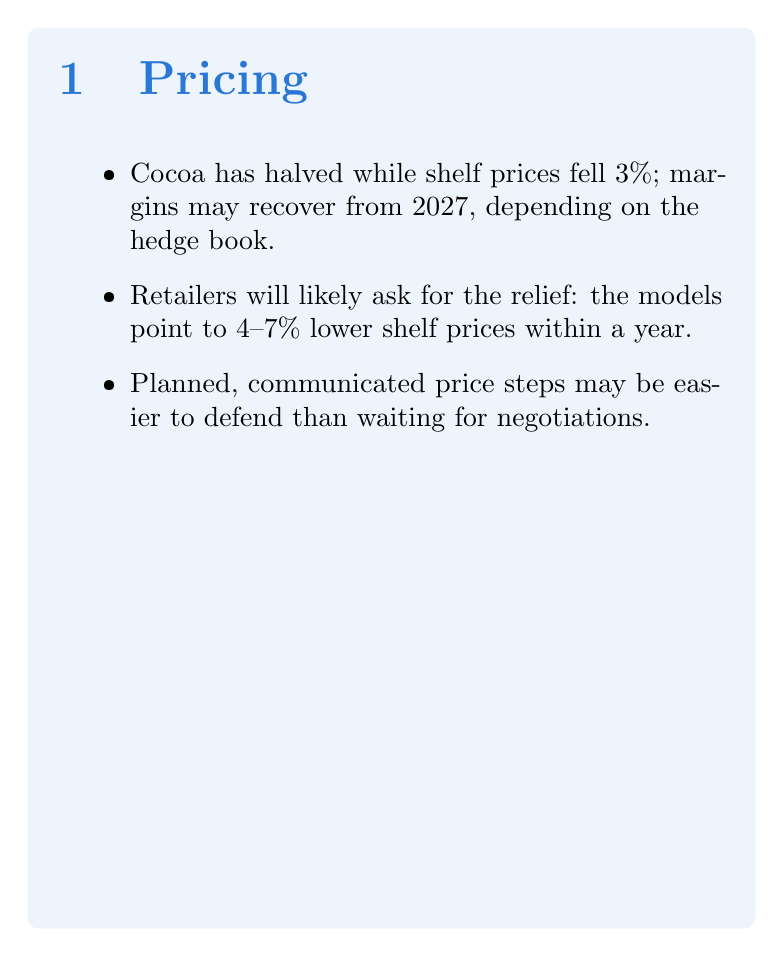
\begin{tikzpicture}\node[fill=tint,rounded corners=4pt,inner sep=12pt,anchor=north]{\parbox[t][106mm][t]{84mm}{%
{\fontsize{19}{23}\selectfont\bfseries\color{blue}1\quad Pricing\par}\vspace{10pt}
\begin{itemize}
\item Cocoa has halved while shelf prices fell 3\%; margins may recover from 2027, depending on the hedge book.
\item Retailers will likely ask for the relief: the models point to 4--7\% lower shelf prices within a year.
\item Planned, communicated price steps may be easier to defend than waiting for negotiations.
\end{itemize}}};\end{tikzpicture}
\end{minipage}\hfill
\begin{minipage}[t]{94mm}\vspace{0pt}
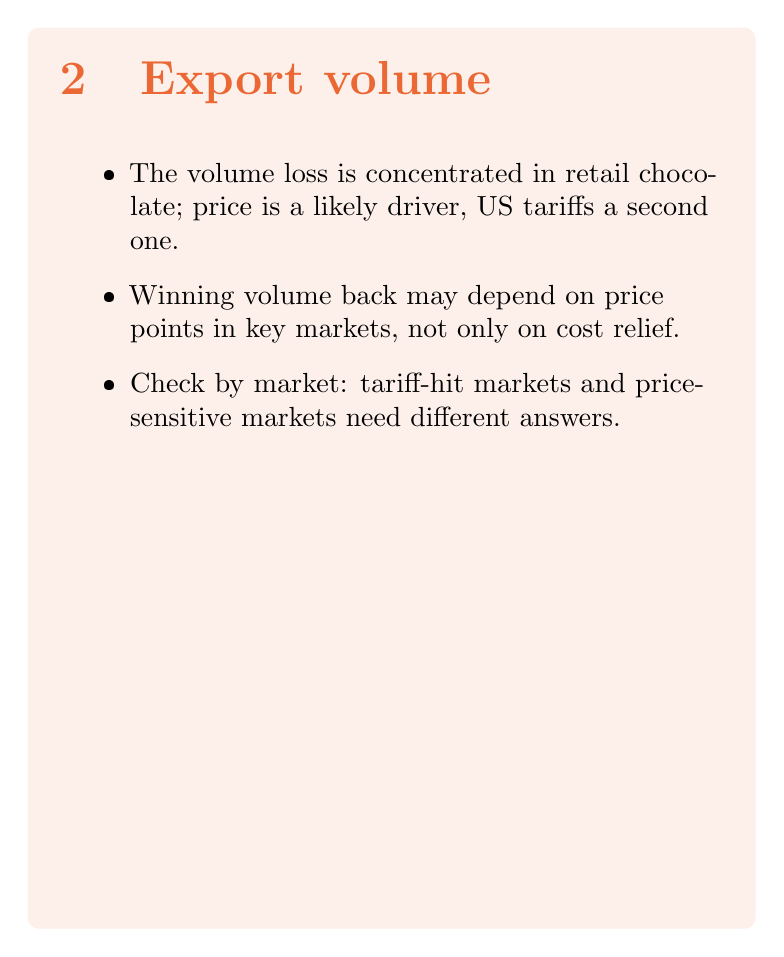
\begin{tikzpicture}\node[fill=tintor,rounded corners=4pt,inner sep=12pt,anchor=north]{\parbox[t][106mm][t]{84mm}{%
{\fontsize{19}{23}\selectfont\bfseries\color{orange}2\quad Export volume\par}\vspace{10pt}
\begin{itemize}
\item The volume loss is concentrated in retail chocolate; price is a likely driver, US tariffs a second one.
\item Winning volume back may depend on price points in key markets, not only on cost relief.
\item Check by market: tariff-hit markets and price-sensitive markets need different answers.
\end{itemize}}};\end{tikzpicture}
\end{minipage}\hfill
\begin{minipage}[t]{94mm}\vspace{0pt}
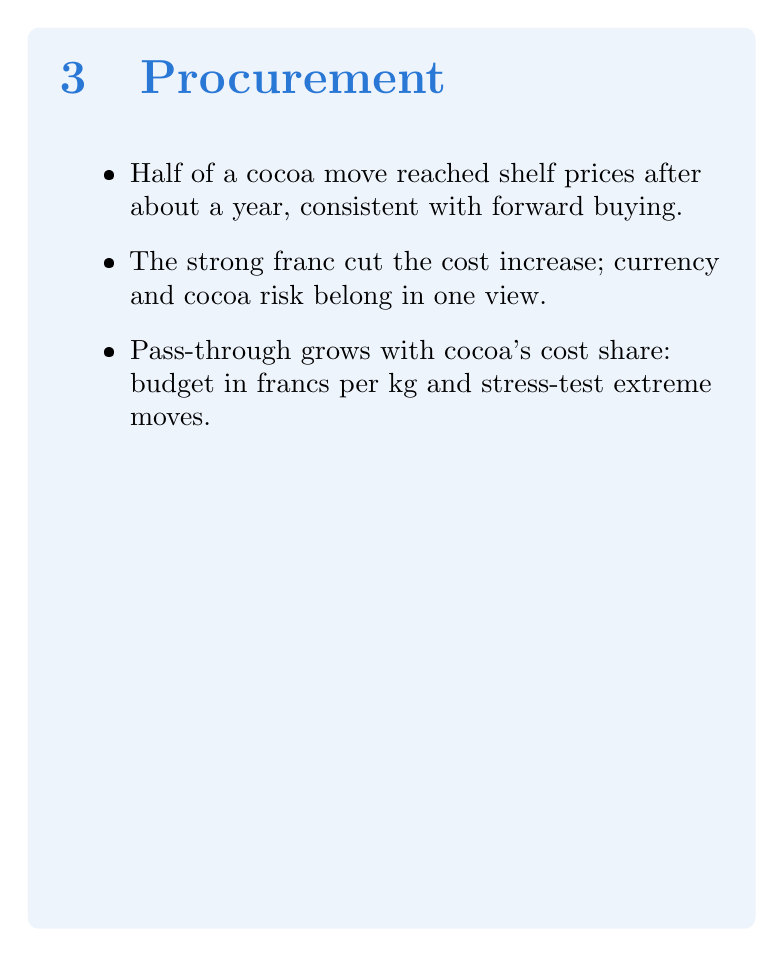
\begin{tikzpicture}\node[fill=tint,rounded corners=4pt,inner sep=12pt,anchor=north]{\parbox[t][106mm][t]{84mm}{%
{\fontsize{19}{23}\selectfont\bfseries\color{blue}3\quad Procurement\par}\vspace{10pt}
\begin{itemize}
\item Half of a cocoa move reached shelf prices after about a year, consistent with forward buying.
\item The strong franc cut the cost increase; currency and cocoa risk belong in one view.
\item Pass-through grows with cocoa's cost share: budget in francs per kg and stress-test extreme moves.
\end{itemize}}};\end{tikzpicture}
\end{minipage}}

% ================= 10 METHODS =================
\slide{Approach, data and limitations}{Full code, data and result tables: github.com/johenmar (repository cocoa-shock-switzerland). AI assistance was used for drafting code and slides; all numbers come from the scripts.}{%
\begin{minipage}[t]{146mm}\vspace{0pt}
{\bfseries Data (monthly)\par}\vspace{6pt}
{\fontsize{13.5}{18}\selectfont
\begin{tabularx}{\linewidth}{@{}lX@{}}
Cocoa price & World Bank Pink Sheet (ICCO indicator), USD/kg, CC BY 4.0\\
Exchange rate & SNB, CHF per USD, monthly average\\
Consumer prices & BFS, LIK detailed indices since 1982 (Dec 2025 = 100)\\
Exports, imports & BAZG, chain-linked unit value and volume indices by CPA, since 2012\\
\end{tabularx}\par}\vspace{12pt}
{\bfseries Methods\par}\vspace{6pt}
{\fontsize{13.5}{18}\selectfont
\begin{itemize}
\item Distributed-lag regression in log changes (24 monthly lags), Newey--West SE; alternative ``franc model'' in CHF changes relative to the shelf price
\item Backtest fitted to Dec 2023, conditional on actual cocoa prices; projection to Aug 2027 with parameter uncertainty
\item Sensitivity: 18/30 lags, sugar prices, no food control, USD prices, pre-2023 sample: 0.9--1.3\% per 10\%
\end{itemize}\par}
\end{minipage}\hfill
\begin{minipage}[t]{146mm}\vspace{0pt}
{\bfseries Limitations\par}\vspace{6pt}
{\fontsize{13.5}{18}\selectfont
\begin{itemize}
\item \textbf{Aggregate data.} No company costs, contracts or hedges; the implications are hypotheses.
\item \textbf{Shelf prices} include imported chocolate and promotions; unit values mix product types.
\item \textbf{Model uncertainty.} The percentage model underestimated this shock; plain OLS intervals are about twice as wide as Newey--West ones.
\item \textbf{Other costs} (milk, sugar, energy, wages) are only partly controlled through food prices.
\item \textbf{Provisional data.} BAZG values for 2026 may be revised.
\end{itemize}\par}
\end{minipage}}

\end{document}
